\setcounter{definition}{0} \setcounter{property}{0} \setcounter{claim}{0} \setcounter{fact}{0} \setcounter{corollary}{0} \setcounter{figure}{0}
\section{Directed Acyclic Graphs}

%For directed graphs, $\{v_j \mid visited[j] = k\}$
%are not necessarily form a connected component~(although you can still run DFS on directed graphs). 
To prepare revealing the connectivity-structure of directed graphs, we first introduce
a spsecial class of directed graphs, directed acyclic graphs~(DAGs).

\begin{definition}[DAG]
A directed graph $G = (V, E)$ is \emph{acyclic} if and only if $G$ does not contain cycles.
\end{definition}

Let $G = (V, E)$ be a directed graph. 
If a vertex $v\in V$ does not have any in-edges~(i.e., \emph{in-degree} is 0), we call it \emph{source vertex};
if a vertex $v\in V$ does not have any out-edges~(i.e., \emph{out-degree} is 0), we call it \emph{sink vertex}.

A directed graph may contain multiple source vertices or sink vertices,
or may not have any source vertex or sink vertex. (Can you give such examples?)

\begin{claim}
A DAG $G=(V,E)$ always has source vertex and sink vertex.
\end{claim}
\emph{Proof.} Let's prove it by contradiction. Assume that $G$ does not contain any source.
First, $G$ must not contain self-loop as otherwise $G$ won't be a DAG.
Let $v$ be any vertex in $V$. As $v$ is not a source, we know that there exists some vertex $u$ points to $v$, i.e., $(u,v)\in E$.
Now since $u$ is not a source then there must exist another vertex $w$ such that $(w,u)\in E$.
Notice that $w \neq v$ as otherwise there will be a cycle: $v = w \to u \to v$.
This means that $w$ is a new vertex. Again as $w$ is not a source, there must exist another \emph{new} vertex points to it.
This process can be extended infinitely following the fact and assumption that $G$ is a DAG and all vertices not are sources,
but this is not possible as the number of vertices is limited. 
The existence of sink can be proved symmetrically. \qed


\begin{definition}[Linearization / Topological Sorting]
Let $G = (V,E)$ be a directed graph. Let $X$ be an ordering of $V$.
If $X$ satisfies: if $(v_i, v_j)\in E$, then $v_i$ is before $v_j$ in $X$,
then we say $X$ is a linearization~(or toplogical sorting) of $G$.
\end{definition}

See some examples below.

\begin{figure}[h!]
\centering{

\tikzset{every picture/.style={line width=0.75pt}} %set default line width to 0.75pt        

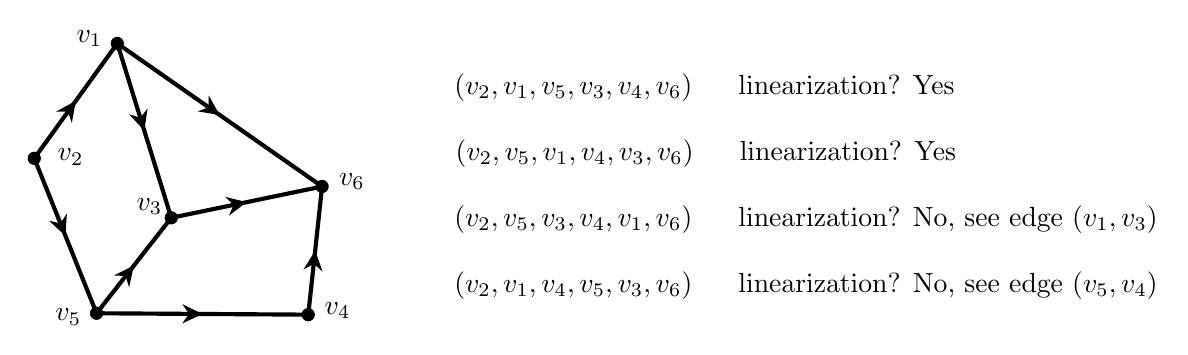
\begin{tikzpicture}[x=0.5pt,y=0.5pt,yscale=-1,xscale=1]
%uncomment if require: \path (0,228); %set diagram left start at 0, and has height of 228

%Flowchart: Connector [id:dp3072392280017706] 
\draw  [fill={rgb, 255:red, 0; green, 0; blue, 0 }  ,fill opacity=1 ] (78,14) .. controls (78,11.58) and (79.96,9.62) .. (82.38,9.62) .. controls (84.79,9.62) and (86.75,11.58) .. (86.75,14) .. controls (86.75,16.42) and (84.79,18.38) .. (82.38,18.38) .. controls (79.96,18.38) and (78,16.42) .. (78,14) -- cycle ;
%Flowchart: Connector [id:dp21397717392367266] 
\draw  [fill={rgb, 255:red, 0; green, 0; blue, 0 }  ,fill opacity=1 ] (63,209) .. controls (63,206.58) and (64.96,204.62) .. (67.38,204.62) .. controls (69.79,204.62) and (71.75,206.58) .. (71.75,209) .. controls (71.75,211.42) and (69.79,213.38) .. (67.38,213.38) .. controls (64.96,213.38) and (63,211.42) .. (63,209) -- cycle ;
%Flowchart: Connector [id:dp8067973087407497] 
\draw  [fill={rgb, 255:red, 0; green, 0; blue, 0 }  ,fill opacity=1 ] (18,97) .. controls (18,94.58) and (19.96,92.62) .. (22.38,92.62) .. controls (24.79,92.62) and (26.75,94.58) .. (26.75,97) .. controls (26.75,99.42) and (24.79,101.38) .. (22.38,101.38) .. controls (19.96,101.38) and (18,99.42) .. (18,97) -- cycle ;
%Flowchart: Connector [id:dp962987276172525] 
\draw  [fill={rgb, 255:red, 0; green, 0; blue, 0 }  ,fill opacity=1 ] (117,140) .. controls (117,137.58) and (118.96,135.62) .. (121.38,135.62) .. controls (123.79,135.62) and (125.75,137.58) .. (125.75,140) .. controls (125.75,142.42) and (123.79,144.38) .. (121.38,144.38) .. controls (118.96,144.38) and (117,142.42) .. (117,140) -- cycle ;
%Straight Lines [id:da5158988833498211] 
\draw [color={rgb, 255:red, 0; green, 0; blue, 0 }  ,draw opacity=1 ][line width=1.5]    (22.38,97) -- (82.38,14) ;
\draw [shift={(52.38,55.5)}, rotate = 125.86] [fill={rgb, 255:red, 0; green, 0; blue, 0 }  ,fill opacity=1 ][line width=0.08]  [draw opacity=0] (14.56,-6.99) -- (0,0) -- (14.56,6.99) -- (9.67,0) -- cycle    ;
%Straight Lines [id:da26521146489140124] 
\draw [color={rgb, 255:red, 0; green, 0; blue, 0 }  ,draw opacity=1 ][line width=1.5]    (67.38,209) -- (121.38,140) ;
\draw [shift={(94.38,174.5)}, rotate = 128.05] [fill={rgb, 255:red, 0; green, 0; blue, 0 }  ,fill opacity=1 ][line width=0.08]  [draw opacity=0] (14.56,-6.99) -- (0,0) -- (14.56,6.99) -- (9.67,0) -- cycle    ;
%Straight Lines [id:da2524996293078703] 
\draw [color={rgb, 255:red, 0; green, 0; blue, 0 }  ,draw opacity=1 ][line width=1.5]    (121.38,140) -- (82.38,14) ;
\draw [shift={(101.88,77)}, rotate = 252.8] [fill={rgb, 255:red, 0; green, 0; blue, 0 }  ,fill opacity=1 ][line width=0.08]  [draw opacity=0] (14.56,-6.99) -- (0,0) -- (14.56,6.99) -- (9.67,0) -- cycle    ;
%Straight Lines [id:da9962026070016303] 
\draw [color={rgb, 255:red, 0; green, 0; blue, 0 }  ,draw opacity=1 ][line width=1.5]    (67.38,209) -- (22.38,97) ;
\draw [shift={(44.88,153)}, rotate = 248.11] [fill={rgb, 255:red, 0; green, 0; blue, 0 }  ,fill opacity=1 ][line width=0.08]  [draw opacity=0] (14.56,-6.99) -- (0,0) -- (14.56,6.99) -- (9.67,0) -- cycle    ;
%Flowchart: Connector [id:dp1566790029206172] 
\draw  [fill={rgb, 255:red, 0; green, 0; blue, 0 }  ,fill opacity=1 ] (216,210) .. controls (216,207.58) and (217.96,205.62) .. (220.38,205.62) .. controls (222.79,205.62) and (224.75,207.58) .. (224.75,210) .. controls (224.75,212.42) and (222.79,214.38) .. (220.38,214.38) .. controls (217.96,214.38) and (216,212.42) .. (216,210) -- cycle ;
%Straight Lines [id:da5810218256695717] 
\draw [color={rgb, 255:red, 0; green, 0; blue, 0 }  ,draw opacity=1 ][line width=1.5]    (67.38,209) -- (220.38,210) ;
\draw [shift={(143.88,209.5)}, rotate = 180.37] [fill={rgb, 255:red, 0; green, 0; blue, 0 }  ,fill opacity=1 ][line width=0.08]  [draw opacity=0] (14.56,-6.99) -- (0,0) -- (14.56,6.99) -- (9.67,0) -- cycle    ;
%Flowchart: Connector [id:dp3466519048019897] 
\draw  [fill={rgb, 255:red, 0; green, 0; blue, 0 }  ,fill opacity=1 ] (226,117.38) .. controls (226,114.96) and (227.96,113) .. (230.38,113) .. controls (232.79,113) and (234.75,114.96) .. (234.75,117.38) .. controls (234.75,119.79) and (232.79,121.75) .. (230.38,121.75) .. controls (227.96,121.75) and (226,119.79) .. (226,117.38) -- cycle ;
%Straight Lines [id:da9047303683615766] 
\draw [color={rgb, 255:red, 0; green, 0; blue, 0 }  ,draw opacity=1 ][line width=1.5]    (121.38,140) -- (230.38,117.38) ;
\draw [shift={(175.88,128.69)}, rotate = 168.27] [fill={rgb, 255:red, 0; green, 0; blue, 0 }  ,fill opacity=1 ][line width=0.08]  [draw opacity=0] (14.56,-6.99) -- (0,0) -- (14.56,6.99) -- (9.67,0) -- cycle    ;
%Straight Lines [id:da5438432067917516] 
\draw [color={rgb, 255:red, 0; green, 0; blue, 0 }  ,draw opacity=1 ][line width=1.5]    (82.38,14) -- (230.38,117.38) ;
\draw [shift={(156.38,65.69)}, rotate = 214.93] [fill={rgb, 255:red, 0; green, 0; blue, 0 }  ,fill opacity=1 ][line width=0.08]  [draw opacity=0] (14.56,-6.99) -- (0,0) -- (14.56,6.99) -- (9.67,0) -- cycle    ;
%Straight Lines [id:da33002644345566856] 
\draw [color={rgb, 255:red, 0; green, 0; blue, 0 }  ,draw opacity=1 ][line width=1.5]    (220.38,210) -- (230.38,117.38) ;
\draw [shift={(225.38,163.69)}, rotate = 96.16] [fill={rgb, 255:red, 0; green, 0; blue, 0 }  ,fill opacity=1 ][line width=0.08]  [draw opacity=0] (14.56,-6.99) -- (0,0) -- (14.56,6.99) -- (9.67,0) -- cycle    ;

% Text Node
\draw (51,3) node [anchor=north west][inner sep=0.75pt]   [align=left] {$\displaystyle v_{1}$};
% Text Node
\draw (94.38,124.38) node [anchor=north west][inner sep=0.75pt]   [align=left] {$\displaystyle v_{3}$};
% Text Node
\draw (35.75,204) node [anchor=north west][inner sep=0.75pt]   [align=left] {$\displaystyle v_{5}$};
% Text Node
\draw (230.38,199.38) node [anchor=north west][inner sep=0.75pt]   [align=left] {$\displaystyle v_{4}$};
% Text Node
\draw (37.38,88.38) node [anchor=north west][inner sep=0.75pt]   [align=left] {$\displaystyle v_{2}$};
% Text Node
\draw (240.75,106.35) node [anchor=north west][inner sep=0.75pt]   [align=left] {$\displaystyle v_{6}$};
% Text Node
\draw (324,34) node [anchor=north west][inner sep=0.75pt]   [align=left] {$\displaystyle ( v_{2} ,v_{1} ,v_{5} ,v_{3} ,v_{4} ,v_{6})$ \ \ \ \ linearization? Yes};
% Text Node
\draw (325,81.67) node [anchor=north west][inner sep=0.75pt]   [align=left] {$\displaystyle ( v_{2} ,v_{5} ,v_{1} ,v_{4} ,v_{3} ,v_{6})$ \ \ \ \ linearization? Yes};
% Text Node
\draw (324,129.34) node [anchor=north west][inner sep=0.75pt]   [align=left] {$\displaystyle ( v_{2} ,v_{5} ,v_{3} ,v_{4} ,v_{1} ,v_{6})$ \ \ \ \ linearization? No, see edge $\displaystyle ( v_{1} ,v_{3})$};
% Text Node
\draw (324,177) node [anchor=north west][inner sep=0.75pt]   [align=left] {$\displaystyle ( v_{2} ,v_{1} ,v_{4} ,v_{5} ,v_{3} ,v_{6})$ \ \ \ \ linearization? No, see edge $\displaystyle ( v_{5} ,v_{4})$};


\end{tikzpicture}

}
\caption{Examples of linearization.}
\end{figure}

If a directed graph $G$ admits a linearization, then we say $G$ can be \emph{linearized}.
We now show that linearization is an \emph{equivalent} characterization of DAGs.

\begin{claim}
A directed graph $G$ can be linearized if and only if $G$ is a DAG.
\label{claim:dag}
\end{claim}

\emph{Proof.}  Let's first prove that if $G$ can be linearized, then $G$ is a DAG.
This is equivalent to proving its contraposition: if $G$ contains a cycle, then $G$ cannot be linearized.
Suppose that there exists an cycle $v_{i_1} \to v_{i_2} \to \cdots \to v_{i_k} \to v_{i_1}$ in $G$.
Then the linearization $X$ must satisfy that $v_{i_{j}}$ is before $v_{i_{j+1}}$ for all $j = 1, 2, \cdots, k-1$,
and that $v_{i_{k}}$ is before $v_{i_1}$, in $X$. Clearly, this is not possible.

The other side of the statement, i.e., if $G$ is a DAG, then $G$ can be linearized, can be proved constructively.
We will design an algorithm~(see below), that constructs a linearization for any DAG. 
The idea of the algorithm is to iteratively
finds source vertex and removes it and its out-edges.

\begin{minipage}{0.8\textwidth}
	\aaA {7}{Algorithm find-linearization ($G = (V, E)$)}\xxx
	\aab {init $X$ as empty list;}\xxx
	\aaB {4}{while ($G$ is not empty)}\xxx
	\aac {arbitrarily find a source vertex $u$ of $G$;}\xxx
	\aac {add $u$ to the end of $X$;}\xxx
	\aac {update $G$ by removing $u$ and its out-edges;}\xxx
	\aab {end while;}\xxx
	\aaa {end algorithm;}\xxx
\end{minipage}

This algorithm is correct. First, when a vertex $u$ is added to $X$,
it is a source vertex of the current graph, which means that
$\{w\mid (w, u)\in E\}$ is either empty or all of them
have been added to $X$. Second, $X$ will include all vertices.
This is because, a source always exists in a DAG~(as we just proved).
The above algorithm is more a framework, as how we update the graph
is not given specifically, and which affects the running time.

Above algorithm gives a constructive proof that, a DAG can always
be linearized. This completes the proof for the fact that, a directed graph is a DAG if and only if it can be linearized.
\qed

%% \begin{claim}
%% Let $X$ be any linearization of a DAG. Then the first vertex of $X$ is a source vertex and 
%% the last vertex of of $X$ is a sink vertex.
%% \label{claim:source}
%% \end{claim}
%% 
%% \emph{Proof.} Let $v_1$ be the first vertex of $X$. Suppose that $v_1$ is not a source of $X$. 
%% By definition of (not being a) source vertex, there exists $(u,v_1)\in E$. Then by the definition
%% of linearization, we know that $u$ will be before $v_1$ in $X$, contradicting to the fact that
%% $v_1$ is the first element of $X$.
%% The other side can be proved symmetrically. \qed
%% 
%% We can use above algorithm to constructively prove following statement.
%% 
%% \begin{claim}
%% Let $G = (V, E)$ be a DAG. A vertex $u\in V$ is a source if and only if 
%% there exists a linearization $X$ of $G$ such that $u$ is the first vertex in $X$.
%% \end{claim}
%% 
%% \emph{Proof.} We first prove that, if $u$ is a source, then there exists a linearization
%% where $u$ is the first vertex of $X$. We prove it by showing that,
%% we can construct such a linearization $X$. We can use above algorithm,
%% and in its first step, we simply pick $u$. The correctness of above algorithm
%% explains the rest.  The other side is exactly Claim~\ref{claim:source}, which we have proved. \qed

\subsection*{Meta-Graph}

For a directed graph $G = (V,E)$, its structure of connectivity can be represented as a new
directed graph, called \emph{meta-graph}, denoted as $G_M = (V_M, E_M)$.
Each of the vertices of the meta-graph corresponds to a connected component of $G$,
and two vertices $C_i, C_j  \in V_M$ are connected by edge $(C_i, C_j) \in E_M$
if and only if there exists edge $(u,v)\in E$ such that $u\in C_i$ and $v\in C_j$.
An example of meta-graph is given below.

\begin{figure}[h!]
\centering{

\tikzset{every picture/.style={line width=0.75pt}} %set default line width to 0.75pt        

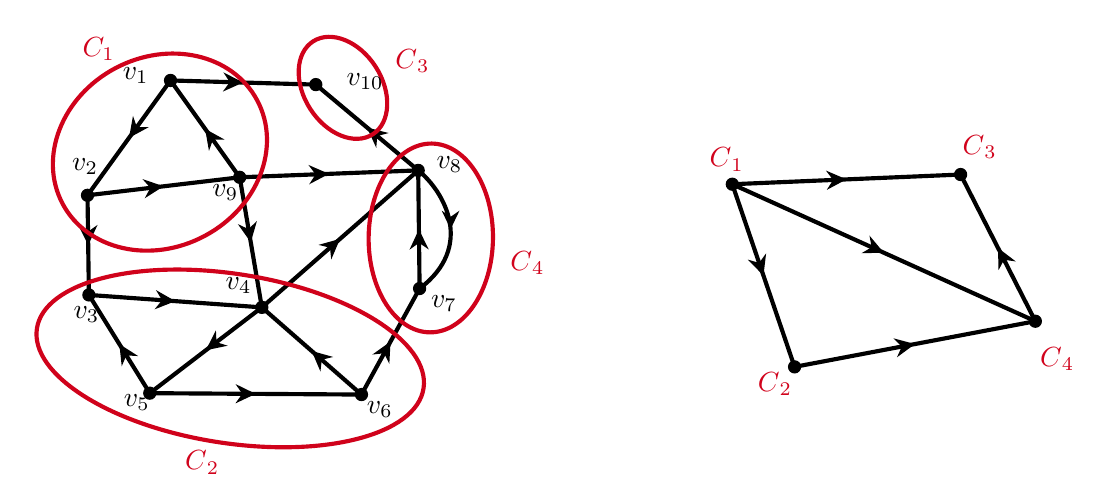
\begin{tikzpicture}[x=0.5pt,y=0.5pt,yscale=-1,xscale=1]
%uncomment if require: \path (0,510); %set diagram left start at 0, and has height of 510

%Flowchart: Connector [id:dp5937668531638635] 
\draw  [fill={rgb, 255:red, 0; green, 0; blue, 0 }  ,fill opacity=1 ] (139,106) .. controls (139,103.58) and (140.96,101.62) .. (143.38,101.62) .. controls (145.79,101.62) and (147.75,103.58) .. (147.75,106) .. controls (147.75,108.42) and (145.79,110.38) .. (143.38,110.38) .. controls (140.96,110.38) and (139,108.42) .. (139,106) -- cycle ;
%Flowchart: Connector [id:dp6657935561963445] 
\draw  [fill={rgb, 255:red, 0; green, 0; blue, 0 }  ,fill opacity=1 ] (244,109) .. controls (244,106.58) and (245.96,104.62) .. (248.38,104.62) .. controls (250.79,104.62) and (252.75,106.58) .. (252.75,109) .. controls (252.75,111.42) and (250.79,113.38) .. (248.38,113.38) .. controls (245.96,113.38) and (244,111.42) .. (244,109) -- cycle ;
%Flowchart: Connector [id:dp14354113795738999] 
\draw  [fill={rgb, 255:red, 0; green, 0; blue, 0 }  ,fill opacity=1 ] (124,332) .. controls (124,329.58) and (125.96,327.62) .. (128.38,327.62) .. controls (130.79,327.62) and (132.75,329.58) .. (132.75,332) .. controls (132.75,334.42) and (130.79,336.38) .. (128.38,336.38) .. controls (125.96,336.38) and (124,334.42) .. (124,332) -- cycle ;
%Flowchart: Connector [id:dp3081556962622095] 
\draw  [fill={rgb, 255:red, 0; green, 0; blue, 0 }  ,fill opacity=1 ] (79,189) .. controls (79,186.58) and (80.96,184.62) .. (83.38,184.62) .. controls (85.79,184.62) and (87.75,186.58) .. (87.75,189) .. controls (87.75,191.42) and (85.79,193.38) .. (83.38,193.38) .. controls (80.96,193.38) and (79,191.42) .. (79,189) -- cycle ;
%Flowchart: Connector [id:dp20013554043379078] 
\draw  [fill={rgb, 255:red, 0; green, 0; blue, 0 }  ,fill opacity=1 ] (189,176) .. controls (189,173.58) and (190.96,171.62) .. (193.38,171.62) .. controls (195.79,171.62) and (197.75,173.58) .. (197.75,176) .. controls (197.75,178.42) and (195.79,180.38) .. (193.38,180.38) .. controls (190.96,180.38) and (189,178.42) .. (189,176) -- cycle ;
%Straight Lines [id:da8865551056781525] 
\draw [color={rgb, 255:red, 0; green, 0; blue, 0 }  ,draw opacity=1 ][line width=1.5]    (83.38,189) -- (143.38,106) ;
\draw [shift={(113.38,147.5)}, rotate = 305.86] [fill={rgb, 255:red, 0; green, 0; blue, 0 }  ,fill opacity=1 ][line width=0.08]  [draw opacity=0] (14.56,-6.99) -- (0,0) -- (14.56,6.99) -- (9.67,0) -- cycle    ;
%Straight Lines [id:da4408247919919335] 
\draw [color={rgb, 255:red, 0; green, 0; blue, 0 }  ,draw opacity=1 ][line width=1.5]    (128.38,332) -- (209.38,270) ;
\draw [shift={(168.88,301)}, rotate = 322.57] [fill={rgb, 255:red, 0; green, 0; blue, 0 }  ,fill opacity=1 ][line width=0.08]  [draw opacity=0] (14.56,-6.99) -- (0,0) -- (14.56,6.99) -- (9.67,0) -- cycle    ;
%Straight Lines [id:da8012008000621113] 
\draw [color={rgb, 255:red, 0; green, 0; blue, 0 }  ,draw opacity=1 ][line width=1.5]    (193.38,176) -- (83.38,189) ;
\draw [shift={(138.38,182.5)}, rotate = 173.26] [fill={rgb, 255:red, 0; green, 0; blue, 0 }  ,fill opacity=1 ][line width=0.08]  [draw opacity=0] (14.56,-6.99) -- (0,0) -- (14.56,6.99) -- (9.67,0) -- cycle    ;
%Straight Lines [id:da01269837290493725] 
\draw [color={rgb, 255:red, 0; green, 0; blue, 0 }  ,draw opacity=1 ][line width=1.5]    (128.38,332) -- (84.38,261) ;
\draw [shift={(106.38,296.5)}, rotate = 418.21000000000004] [fill={rgb, 255:red, 0; green, 0; blue, 0 }  ,fill opacity=1 ][line width=0.08]  [draw opacity=0] (14.56,-6.99) -- (0,0) -- (14.56,6.99) -- (9.67,0) -- cycle    ;
%Flowchart: Connector [id:dp01738972677326256] 
\draw  [fill={rgb, 255:red, 0; green, 0; blue, 0 }  ,fill opacity=1 ] (277,333) .. controls (277,330.58) and (278.96,328.62) .. (281.38,328.62) .. controls (283.79,328.62) and (285.75,330.58) .. (285.75,333) .. controls (285.75,335.42) and (283.79,337.38) .. (281.38,337.38) .. controls (278.96,337.38) and (277,335.42) .. (277,333) -- cycle ;
%Straight Lines [id:da9151099863353562] 
\draw [color={rgb, 255:red, 0; green, 0; blue, 0 }  ,draw opacity=1 ][line width=1.5]    (281.38,333) -- (323.38,256.38) ;
\draw [shift={(302.38,294.69)}, rotate = 478.73] [fill={rgb, 255:red, 0; green, 0; blue, 0 }  ,fill opacity=1 ][line width=0.08]  [draw opacity=0] (14.56,-6.99) -- (0,0) -- (14.56,6.99) -- (9.67,0) -- cycle    ;
%Straight Lines [id:da8589700496158776] 
\draw [color={rgb, 255:red, 0; green, 0; blue, 0 }  ,draw opacity=1 ][line width=1.5]    (128.38,332) -- (281.38,333) ;
\draw [shift={(204.88,332.5)}, rotate = 180.37] [fill={rgb, 255:red, 0; green, 0; blue, 0 }  ,fill opacity=1 ][line width=0.08]  [draw opacity=0] (14.56,-6.99) -- (0,0) -- (14.56,6.99) -- (9.67,0) -- cycle    ;
%Flowchart: Connector [id:dp23564521467293476] 
\draw  [fill={rgb, 255:red, 0; green, 0; blue, 0 }  ,fill opacity=1 ] (319,256.38) .. controls (319,253.96) and (320.96,252) .. (323.38,252) .. controls (325.79,252) and (327.75,253.96) .. (327.75,256.38) .. controls (327.75,258.79) and (325.79,260.75) .. (323.38,260.75) .. controls (320.96,260.75) and (319,258.79) .. (319,256.38) -- cycle ;
%Straight Lines [id:da5765902383361479] 
\draw [color={rgb, 255:red, 0; green, 0; blue, 0 }  ,draw opacity=1 ][line width=1.5]    (323.38,256.38) -- (322.38,171) ;
\draw [shift={(322.88,213.69)}, rotate = 449.33] [fill={rgb, 255:red, 0; green, 0; blue, 0 }  ,fill opacity=1 ][line width=0.08]  [draw opacity=0] (14.56,-6.99) -- (0,0) -- (14.56,6.99) -- (9.67,0) -- cycle    ;
%Straight Lines [id:da6859280233883376] 
\draw [color={rgb, 255:red, 0; green, 0; blue, 0 }  ,draw opacity=1 ][line width=1.5]    (322.38,171) -- (248.38,109) ;
\draw [shift={(285.38,140)}, rotate = 399.96000000000004] [fill={rgb, 255:red, 0; green, 0; blue, 0 }  ,fill opacity=1 ][line width=0.08]  [draw opacity=0] (14.56,-6.99) -- (0,0) -- (14.56,6.99) -- (9.67,0) -- cycle    ;
%Straight Lines [id:da329141247373788] 
\draw [color={rgb, 255:red, 0; green, 0; blue, 0 }  ,draw opacity=1 ][line width=1.5]    (143.38,106) -- (193.38,176) ;
\draw [shift={(168.38,141)}, rotate = 54.46] [fill={rgb, 255:red, 0; green, 0; blue, 0 }  ,fill opacity=1 ][line width=0.08]  [draw opacity=0] (14.56,-6.99) -- (0,0) -- (14.56,6.99) -- (9.67,0) -- cycle    ;
%Straight Lines [id:da25009890870323437] 
\draw [color={rgb, 255:red, 0; green, 0; blue, 0 }  ,draw opacity=1 ][line width=1.5]    (209.38,270) -- (281.38,333) ;
\draw [shift={(245.38,301.5)}, rotate = 41.19] [fill={rgb, 255:red, 0; green, 0; blue, 0 }  ,fill opacity=1 ][line width=0.08]  [draw opacity=0] (14.56,-6.99) -- (0,0) -- (14.56,6.99) -- (9.67,0) -- cycle    ;
%Flowchart: Connector [id:dp20561620581532858] 
\draw  [fill={rgb, 255:red, 0; green, 0; blue, 0 }  ,fill opacity=1 ] (205,270) .. controls (205,267.58) and (206.96,265.62) .. (209.38,265.62) .. controls (211.79,265.62) and (213.75,267.58) .. (213.75,270) .. controls (213.75,272.42) and (211.79,274.38) .. (209.38,274.38) .. controls (206.96,274.38) and (205,272.42) .. (205,270) -- cycle ;
%Flowchart: Connector [id:dp4014605163661533] 
\draw  [fill={rgb, 255:red, 0; green, 0; blue, 0 }  ,fill opacity=1 ] (80,261) .. controls (80,258.58) and (81.96,256.62) .. (84.38,256.62) .. controls (86.79,256.62) and (88.75,258.58) .. (88.75,261) .. controls (88.75,263.42) and (86.79,265.38) .. (84.38,265.38) .. controls (81.96,265.38) and (80,263.42) .. (80,261) -- cycle ;
%Flowchart: Connector [id:dp14845565107772662] 
\draw  [fill={rgb, 255:red, 0; green, 0; blue, 0 }  ,fill opacity=1 ] (318,171) .. controls (318,168.58) and (319.96,166.62) .. (322.38,166.62) .. controls (324.79,166.62) and (326.75,168.58) .. (326.75,171) .. controls (326.75,173.42) and (324.79,175.38) .. (322.38,175.38) .. controls (319.96,175.38) and (318,173.42) .. (318,171) -- cycle ;
%Straight Lines [id:da3881378688310262] 
\draw [color={rgb, 255:red, 0; green, 0; blue, 0 }  ,draw opacity=1 ][line width=1.5]    (209.38,270) -- (84.38,261) ;
\draw [shift={(146.88,265.5)}, rotate = 184.12] [fill={rgb, 255:red, 0; green, 0; blue, 0 }  ,fill opacity=1 ][line width=0.08]  [draw opacity=0] (14.56,-6.99) -- (0,0) -- (14.56,6.99) -- (9.67,0) -- cycle    ;
%Curve Lines [id:da8015709651805362] 
\draw [line width=1.5]    (323.38,256.38) .. controls (363.38,226.38) and (341.68,186.52) .. (322.38,171) ;
\draw [shift={(345.77,213.48)}, rotate = 270.05] [fill={rgb, 255:red, 0; green, 0; blue, 0 }  ][line width=0.08]  [draw opacity=0] (13.4,-6.43) -- (0,0) -- (13.4,6.44) -- (8.9,0) -- cycle    ;
%Straight Lines [id:da4386825484478063] 
\draw [color={rgb, 255:red, 0; green, 0; blue, 0 }  ,draw opacity=1 ][line width=1.5]    (209.38,270) -- (322.38,171) ;
\draw [shift={(265.88,220.5)}, rotate = 498.78] [fill={rgb, 255:red, 0; green, 0; blue, 0 }  ,fill opacity=1 ][line width=0.08]  [draw opacity=0] (14.56,-6.99) -- (0,0) -- (14.56,6.99) -- (9.67,0) -- cycle    ;
%Straight Lines [id:da26616639892534444] 
\draw [color={rgb, 255:red, 0; green, 0; blue, 0 }  ,draw opacity=1 ][line width=1.5]    (193.38,176) -- (209.38,270) ;
\draw [shift={(201.38,223)}, rotate = 260.34000000000003] [fill={rgb, 255:red, 0; green, 0; blue, 0 }  ,fill opacity=1 ][line width=0.08]  [draw opacity=0] (14.56,-6.99) -- (0,0) -- (14.56,6.99) -- (9.67,0) -- cycle    ;
%Straight Lines [id:da34500416847135773] 
\draw [color={rgb, 255:red, 0; green, 0; blue, 0 }  ,draw opacity=1 ][line width=1.5]    (83.38,189) -- (84.38,261) ;
\draw [shift={(83.88,225)}, rotate = 269.2] [fill={rgb, 255:red, 0; green, 0; blue, 0 }  ,fill opacity=1 ][line width=0.08]  [draw opacity=0] (14.56,-6.99) -- (0,0) -- (14.56,6.99) -- (9.67,0) -- cycle    ;
%Straight Lines [id:da4267721016610234] 
\draw [color={rgb, 255:red, 0; green, 0; blue, 0 }  ,draw opacity=1 ][line width=1.5]    (193.38,176) -- (322.38,171) ;
\draw [shift={(257.88,173.5)}, rotate = 537.78] [fill={rgb, 255:red, 0; green, 0; blue, 0 }  ,fill opacity=1 ][line width=0.08]  [draw opacity=0] (14.56,-6.99) -- (0,0) -- (14.56,6.99) -- (9.67,0) -- cycle    ;
%Straight Lines [id:da8164594223234878] 
\draw [color={rgb, 255:red, 0; green, 0; blue, 0 }  ,draw opacity=1 ][line width=1.5]    (143.38,106) -- (248.38,109) ;
\draw [shift={(195.88,107.5)}, rotate = 181.64] [fill={rgb, 255:red, 0; green, 0; blue, 0 }  ,fill opacity=1 ][line width=0.08]  [draw opacity=0] (14.56,-6.99) -- (0,0) -- (14.56,6.99) -- (9.67,0) -- cycle    ;
%Shape: Ellipse [id:dp27109176732345586] 
\draw  [color={rgb, 255:red, 208; green, 2; blue, 27 }  ,draw opacity=1 ][line width=1.5]  (65.39,195.12) .. controls (47.61,161.62) and (64.68,117.75) .. (103.52,97.13) .. controls (142.37,76.52) and (188.27,86.96) .. (206.05,120.45) .. controls (223.83,153.95) and (206.76,197.82) .. (167.91,218.44) .. controls (129.07,239.06) and (83.17,228.61) .. (65.39,195.12) -- cycle ;
%Shape: Ellipse [id:dp0877469193537469] 
\draw  [color={rgb, 255:red, 208; green, 2; blue, 27 }  ,draw opacity=1 ][line width=1.5]  (46.82,285.18) .. controls (52.01,251.81) and (118.75,234.47) .. (195.91,246.46) .. controls (273.06,258.44) and (331.4,295.21) .. (326.22,328.58) .. controls (321.04,361.95) and (254.29,379.29) .. (177.14,367.3) .. controls (99.98,355.32) and (41.64,318.55) .. (46.82,285.18) -- cycle ;
%Shape: Ellipse [id:dp6318272598845582] 
\draw  [color={rgb, 255:red, 208; green, 2; blue, 27 }  ,draw opacity=1 ][line width=1.5]  (332.2,151.61) .. controls (357.02,151.88) and (376.8,182.63) .. (376.4,220.31) .. controls (376,257.98) and (355.56,288.31) .. (330.75,288.04) .. controls (305.94,287.78) and (286.15,257.02) .. (286.55,219.35) .. controls (286.96,181.68) and (307.39,151.35) .. (332.2,151.61) -- cycle ;
%Shape: Ellipse [id:dp1869855316402914] 
\draw  [color={rgb, 255:red, 208; green, 2; blue, 27 }  ,draw opacity=1 ][line width=1.5]  (246.45,77.74) .. controls (259.53,69.36) and (279.77,77.6) .. (291.66,96.15) .. controls (303.55,114.71) and (302.58,136.54) .. (289.5,144.92) .. controls (276.42,153.3) and (256.19,145.05) .. (244.3,126.5) .. controls (232.41,107.95) and (233.38,86.12) .. (246.45,77.74) -- cycle ;
%Flowchart: Connector [id:dp51888588365958] 
\draw  [fill={rgb, 255:red, 0; green, 0; blue, 0 }  ,fill opacity=1 ] (590,313) .. controls (590,310.58) and (591.96,308.62) .. (594.38,308.62) .. controls (596.79,308.62) and (598.75,310.58) .. (598.75,313) .. controls (598.75,315.42) and (596.79,317.38) .. (594.38,317.38) .. controls (591.96,317.38) and (590,315.42) .. (590,313) -- cycle ;
%Straight Lines [id:da6410921260405182] 
\draw [color={rgb, 255:red, 0; green, 0; blue, 0 }  ,draw opacity=1 ][line width=1.5]    (768.38,280) -- (549.38,181) ;
\draw [shift={(658.88,230.5)}, rotate = 204.33] [fill={rgb, 255:red, 0; green, 0; blue, 0 }  ,fill opacity=1 ][line width=0.08]  [draw opacity=0] (14.56,-6.99) -- (0,0) -- (14.56,6.99) -- (9.67,0) -- cycle    ;
%Straight Lines [id:da8627356399127929] 
\draw [color={rgb, 255:red, 0; green, 0; blue, 0 }  ,draw opacity=1 ][line width=1.5]    (768.38,280) -- (714.38,174) ;
\draw [shift={(741.38,227)}, rotate = 423] [fill={rgb, 255:red, 0; green, 0; blue, 0 }  ,fill opacity=1 ][line width=0.08]  [draw opacity=0] (14.56,-6.99) -- (0,0) -- (14.56,6.99) -- (9.67,0) -- cycle    ;
%Flowchart: Connector [id:dp5660576336850748] 
\draw  [fill={rgb, 255:red, 0; green, 0; blue, 0 }  ,fill opacity=1 ] (710,174) .. controls (710,171.58) and (711.96,169.62) .. (714.38,169.62) .. controls (716.79,169.62) and (718.75,171.58) .. (718.75,174) .. controls (718.75,176.42) and (716.79,178.38) .. (714.38,178.38) .. controls (711.96,178.38) and (710,176.42) .. (710,174) -- cycle ;
%Flowchart: Connector [id:dp5784688617216504] 
\draw  [fill={rgb, 255:red, 0; green, 0; blue, 0 }  ,fill opacity=1 ] (545,181) .. controls (545,178.58) and (546.96,176.62) .. (549.38,176.62) .. controls (551.79,176.62) and (553.75,178.58) .. (553.75,181) .. controls (553.75,183.42) and (551.79,185.38) .. (549.38,185.38) .. controls (546.96,185.38) and (545,183.42) .. (545,181) -- cycle ;
%Straight Lines [id:da35390930720516367] 
\draw [color={rgb, 255:red, 0; green, 0; blue, 0 }  ,draw opacity=1 ][line width=1.5]    (594.38,313) -- (549.38,181) ;
\draw [shift={(571.88,247)}, rotate = 251.18] [fill={rgb, 255:red, 0; green, 0; blue, 0 }  ,fill opacity=1 ][line width=0.08]  [draw opacity=0] (14.56,-6.99) -- (0,0) -- (14.56,6.99) -- (9.67,0) -- cycle    ;
%Straight Lines [id:da16486738526478106] 
\draw [color={rgb, 255:red, 0; green, 0; blue, 0 }  ,draw opacity=1 ][line width=1.5]    (549.38,181) -- (714.38,174) ;
\draw [shift={(631.88,177.5)}, rotate = 537.5699999999999] [fill={rgb, 255:red, 0; green, 0; blue, 0 }  ,fill opacity=1 ][line width=0.08]  [draw opacity=0] (14.56,-6.99) -- (0,0) -- (14.56,6.99) -- (9.67,0) -- cycle    ;
%Flowchart: Connector [id:dp49963370359380055] 
\draw  [fill={rgb, 255:red, 0; green, 0; blue, 0 }  ,fill opacity=1 ] (764,280) .. controls (764,277.58) and (765.96,275.62) .. (768.38,275.62) .. controls (770.79,275.62) and (772.75,277.58) .. (772.75,280) .. controls (772.75,282.42) and (770.79,284.38) .. (768.38,284.38) .. controls (765.96,284.38) and (764,282.42) .. (764,280) -- cycle ;
%Straight Lines [id:da8408093021248022] 
\draw [color={rgb, 255:red, 0; green, 0; blue, 0 }  ,draw opacity=1 ][line width=1.5]    (768.38,280) -- (594.38,313) ;
\draw [shift={(681.38,296.5)}, rotate = 169.26] [fill={rgb, 255:red, 0; green, 0; blue, 0 }  ,fill opacity=1 ][line width=0.08]  [draw opacity=0] (14.56,-6.99) -- (0,0) -- (14.56,6.99) -- (9.67,0) -- cycle    ;

% Text Node
\draw (107,94.93) node [anchor=north west][inner sep=0.75pt]   [align=left] {$\displaystyle v_{1}$};
% Text Node
\draw (71.38,267.31) node [anchor=north west][inner sep=0.75pt]   [align=left] {$\displaystyle v_{3}$};
% Text Node
\draw (107.75,330.93) node [anchor=north west][inner sep=0.75pt]   [align=left] {$\displaystyle v_{5}$};
% Text Node
\draw (181.38,246.31) node [anchor=north west][inner sep=0.75pt]   [align=left] {$\displaystyle v_{4}$};
% Text Node
\draw (70.38,160.31) node [anchor=north west][inner sep=0.75pt]   [align=left] {$\displaystyle v_{2}$};
% Text Node
\draw (171.75,179.29) node [anchor=north west][inner sep=0.75pt]   [align=left] {$\displaystyle v_{9}$};
% Text Node
\draw (329.75,259.31) node [anchor=north west][inner sep=0.75pt]   [align=left] {$\displaystyle v_{7}$};
% Text Node
\draw (283.38,335.93) node [anchor=north west][inner sep=0.75pt]   [align=left] {$\displaystyle v_{6}$};
% Text Node
\draw (333.75,159.29) node [anchor=north west][inner sep=0.75pt]   [align=left] {$\displaystyle v_{8}$};
% Text Node
\draw (268.75,99.29) node [anchor=north west][inner sep=0.75pt]   [align=left] {$\displaystyle v_{10}$};
% Text Node
\draw (78,72.93) node [anchor=north west][inner sep=0.75pt]   [align=left] {$\displaystyle \textcolor[rgb]{0.82,0.01,0.11}{C_{1}}$};
% Text Node
\draw (152,371.93) node [anchor=north west][inner sep=0.75pt]   [align=left] {$\displaystyle \textcolor[rgb]{0.82,0.01,0.11}{C}\textcolor[rgb]{0.82,0.01,0.11}{_{2}}$};
% Text Node
\draw (387,227.93) node [anchor=north west][inner sep=0.75pt]   [align=left] {$\displaystyle \textcolor[rgb]{0.82,0.01,0.11}{C}\textcolor[rgb]{0.82,0.01,0.11}{_{4}}$};
% Text Node
\draw (304,81.93) node [anchor=north west][inner sep=0.75pt]   [align=left] {$\displaystyle \textcolor[rgb]{0.82,0.01,0.11}{C}\textcolor[rgb]{0.82,0.01,0.11}{_{3}}$};
% Text Node
\draw (566,314.93) node [anchor=north west][inner sep=0.75pt]   [align=left] {$\displaystyle \textcolor[rgb]{0.82,0.01,0.11}{C}\textcolor[rgb]{0.82,0.01,0.11}{_{2}}$};
% Text Node
\draw (770,296.93) node [anchor=north west][inner sep=0.75pt]   [align=left] {$\displaystyle \textcolor[rgb]{0.82,0.01,0.11}{C}\textcolor[rgb]{0.82,0.01,0.11}{_{4}}$};
% Text Node
\draw (531,152.93) node [anchor=north west][inner sep=0.75pt]   [align=left] {$\displaystyle \textcolor[rgb]{0.82,0.01,0.11}{C}\textcolor[rgb]{0.82,0.01,0.11}{_{1}}$};
% Text Node
\draw (714,143.93) node [anchor=north west][inner sep=0.75pt]   [align=left] {$\displaystyle \textcolor[rgb]{0.82,0.01,0.11}{C}\textcolor[rgb]{0.82,0.01,0.11}{_{3}}$};


\end{tikzpicture}

}
\caption{Example of meta-graph.}
\label{fig:meta-graph}
\end{figure}

Meta-graph has an important property: it does not contain cycles, i.e., it is a directed acyclic graph~(DAG).

\begin{claim}
The meta-graph $G_M$ of any directed graph $G$ is a directed acyclic graph.
\end{claim}

\emph{Proof.} Suppose conversely that $G_M$ contains a cycle, $C_1 \to C_2 \to C_k \to C_1$,
then the union of the vertices in these connected components form a single connected component,
contradicting to the \emph{maximal} property of connected component. \qed

\subsection*{Reverse Graph}

\begin{definition}
Let $G = (V,E)$ be a directed graph. The \emph{reverse graph} of $G$, denoted as $G_R = (V, E_R)$,
has the same set of vertices and edges with reversed direction, i.e., $(u,v) \in E$ if and only if $(v,u)\in E_R$.
\end{definition}

\begin{figure}[!h]
\centering{

\tikzset{every picture/.style={line width=0.75pt}} %set default line width to 0.75pt        

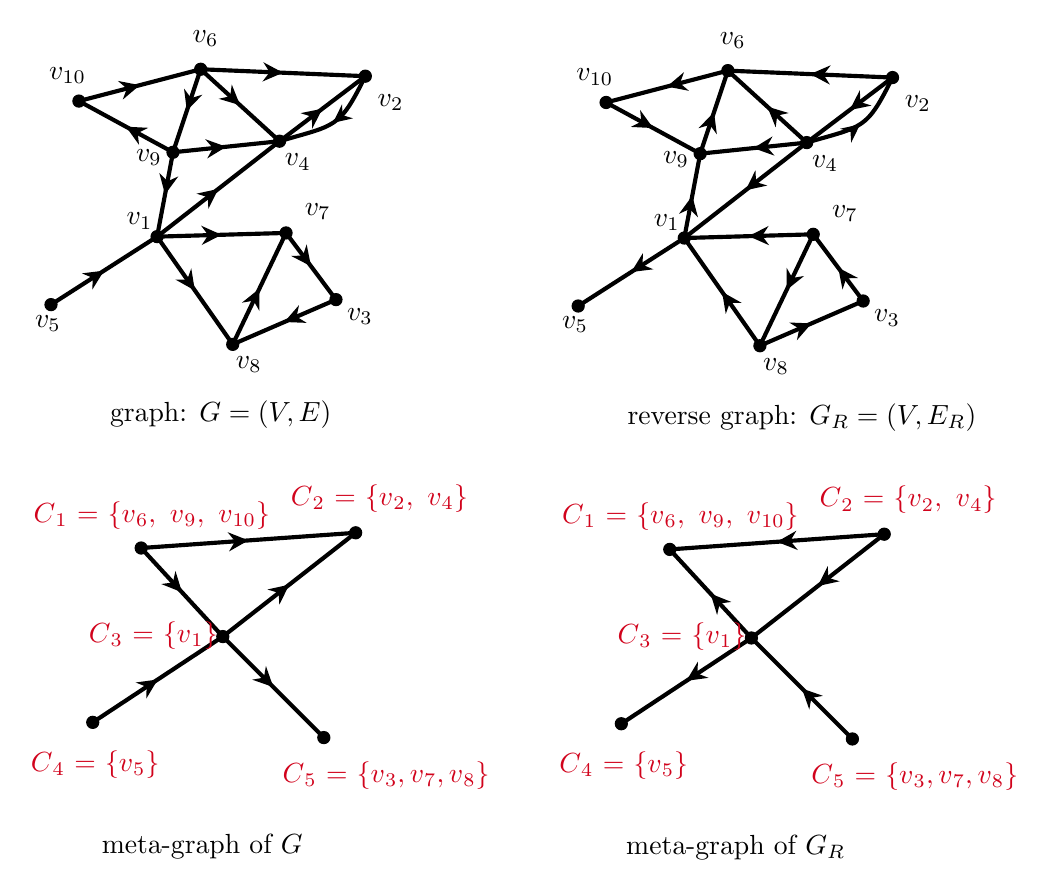
\begin{tikzpicture}[x=0.5pt,y=0.5pt,yscale=-1,xscale=1]
%uncomment if require: \path (0,615); %set diagram left start at 0, and has height of 615

%Flowchart: Connector [id:dp35531003904401826] 
\draw  [fill={rgb, 255:red, 0; green, 0; blue, 0 }  ,fill opacity=1 ] (87,378) .. controls (87,375.58) and (88.96,373.62) .. (91.38,373.62) .. controls (93.79,373.62) and (95.75,375.58) .. (95.75,378) .. controls (95.75,380.42) and (93.79,382.38) .. (91.38,382.38) .. controls (88.96,382.38) and (87,380.42) .. (87,378) -- cycle ;
%Straight Lines [id:da06413387293276729] 
\draw [color={rgb, 255:red, 0; green, 0; blue, 0 }  ,draw opacity=1 ][line width=1.5]    (114.38,92) -- (134.38,32) ;
\draw [shift={(124.38,62)}, rotate = 288.43] [fill={rgb, 255:red, 0; green, 0; blue, 0 }  ,fill opacity=1 ][line width=0.08]  [draw opacity=0] (14.56,-6.99) -- (0,0) -- (14.56,6.99) -- (9.67,0) -- cycle    ;
%Straight Lines [id:da9572573982067856] 
\draw [color={rgb, 255:red, 0; green, 0; blue, 0 }  ,draw opacity=1 ][line width=1.5]    (134.38,32) -- (46.38,55) ;
\draw [shift={(90.38,43.5)}, rotate = 165.35] [fill={rgb, 255:red, 0; green, 0; blue, 0 }  ,fill opacity=1 ][line width=0.08]  [draw opacity=0] (14.56,-6.99) -- (0,0) -- (14.56,6.99) -- (9.67,0) -- cycle    ;
%Straight Lines [id:da027017237295007268] 
\draw [color={rgb, 255:red, 0; green, 0; blue, 0 }  ,draw opacity=1 ][line width=1.5]    (150.38,442) -- (91.38,378) ;
\draw [shift={(120.88,410)}, rotate = 227.33] [fill={rgb, 255:red, 0; green, 0; blue, 0 }  ,fill opacity=1 ][line width=0.08]  [draw opacity=0] (14.56,-6.99) -- (0,0) -- (14.56,6.99) -- (9.67,0) -- cycle    ;
%Flowchart: Connector [id:dp7018202329285442] 
\draw  [fill={rgb, 255:red, 0; green, 0; blue, 0 }  ,fill opacity=1 ] (242,367) .. controls (242,364.58) and (243.96,362.62) .. (246.38,362.62) .. controls (248.79,362.62) and (250.75,364.58) .. (250.75,367) .. controls (250.75,369.42) and (248.79,371.38) .. (246.38,371.38) .. controls (243.96,371.38) and (242,369.42) .. (242,367) -- cycle ;
%Flowchart: Connector [id:dp9468304553677146] 
\draw  [fill={rgb, 255:red, 0; green, 0; blue, 0 }  ,fill opacity=1 ] (249,37) .. controls (249,34.58) and (250.96,32.62) .. (253.38,32.62) .. controls (255.79,32.62) and (257.75,34.58) .. (257.75,37) .. controls (257.75,39.42) and (255.79,41.38) .. (253.38,41.38) .. controls (250.96,41.38) and (249,39.42) .. (249,37) -- cycle ;
%Flowchart: Connector [id:dp10084257988995149] 
\draw  [fill={rgb, 255:red, 0; green, 0; blue, 0 }  ,fill opacity=1 ] (187,84) .. controls (187,81.58) and (188.96,79.62) .. (191.38,79.62) .. controls (193.79,79.62) and (195.75,81.58) .. (195.75,84) .. controls (195.75,86.42) and (193.79,88.38) .. (191.38,88.38) .. controls (188.96,88.38) and (187,86.42) .. (187,84) -- cycle ;
%Flowchart: Connector [id:dp5678652918378437] 
\draw  [fill={rgb, 255:red, 0; green, 0; blue, 0 }  ,fill opacity=1 ] (191.99,148.72) .. controls (192.85,146.46) and (195.39,145.34) .. (197.64,146.21) .. controls (199.9,147.08) and (201.02,149.61) .. (200.15,151.86) .. controls (199.28,154.12) and (196.75,155.24) .. (194.5,154.38) .. controls (192.24,153.51) and (191.12,150.97) .. (191.99,148.72) -- cycle ;
%Flowchart: Connector [id:dp9451957343710085] 
\draw  [fill={rgb, 255:red, 0; green, 0; blue, 0 }  ,fill opacity=1 ] (228.07,196.91) .. controls (228.94,194.66) and (231.47,193.53) .. (233.73,194.4) .. controls (235.98,195.27) and (237.11,197.8) .. (236.24,200.06) .. controls (235.37,202.32) and (232.84,203.44) .. (230.58,202.57) .. controls (228.33,201.7) and (227.2,199.17) .. (228.07,196.91) -- cycle ;
%Flowchart: Connector [id:dp7598246465914121] 
\draw  [fill={rgb, 255:red, 0; green, 0; blue, 0 }  ,fill opacity=1 ] (153.46,229.25) .. controls (154.33,227) and (156.86,225.87) .. (159.11,226.74) .. controls (161.37,227.61) and (162.49,230.14) .. (161.63,232.4) .. controls (160.76,234.65) and (158.22,235.78) .. (155.97,234.91) .. controls (153.71,234.04) and (152.59,231.51) .. (153.46,229.25) -- cycle ;
%Flowchart: Connector [id:dp9270593548114698] 
\draw  [fill={rgb, 255:red, 0; green, 0; blue, 0 }  ,fill opacity=1 ] (22.12,200.53) .. controls (22.99,198.28) and (25.52,197.15) .. (27.77,198.02) .. controls (30.03,198.89) and (31.15,201.42) .. (30.28,203.68) .. controls (29.42,205.94) and (26.88,207.06) .. (24.63,206.19) .. controls (22.37,205.32) and (21.25,202.79) .. (22.12,200.53) -- cycle ;
%Flowchart: Connector [id:dp0003313036349563703] 
\draw  [fill={rgb, 255:red, 0; green, 0; blue, 0 }  ,fill opacity=1 ] (98.79,151.39) .. controls (99.66,149.14) and (102.2,148.01) .. (104.45,148.88) .. controls (106.71,149.75) and (107.83,152.28) .. (106.96,154.54) .. controls (106.09,156.8) and (103.56,157.92) .. (101.3,157.05) .. controls (99.05,156.18) and (97.92,153.65) .. (98.79,151.39) -- cycle ;
%Flowchart: Connector [id:dp05524410597346219] 
\draw  [fill={rgb, 255:red, 0; green, 0; blue, 0 }  ,fill opacity=1 ] (130,32) .. controls (130,29.58) and (131.96,27.62) .. (134.38,27.62) .. controls (136.79,27.62) and (138.75,29.58) .. (138.75,32) .. controls (138.75,34.42) and (136.79,36.38) .. (134.38,36.38) .. controls (131.96,36.38) and (130,34.42) .. (130,32) -- cycle ;
%Flowchart: Connector [id:dp8722833316705884] 
\draw  [fill={rgb, 255:red, 0; green, 0; blue, 0 }  ,fill opacity=1 ] (42,55) .. controls (42,52.58) and (43.96,50.62) .. (46.38,50.62) .. controls (48.79,50.62) and (50.75,52.58) .. (50.75,55) .. controls (50.75,57.42) and (48.79,59.38) .. (46.38,59.38) .. controls (43.96,59.38) and (42,57.42) .. (42,55) -- cycle ;
%Flowchart: Connector [id:dp04902898021909796] 
\draw  [fill={rgb, 255:red, 0; green, 0; blue, 0 }  ,fill opacity=1 ] (110,92) .. controls (110,89.58) and (111.96,87.62) .. (114.38,87.62) .. controls (116.79,87.62) and (118.75,89.58) .. (118.75,92) .. controls (118.75,94.42) and (116.79,96.38) .. (114.38,96.38) .. controls (111.96,96.38) and (110,94.42) .. (110,92) -- cycle ;
%Straight Lines [id:da6957258198444844] 
\draw [color={rgb, 255:red, 0; green, 0; blue, 0 }  ,draw opacity=1 ][line width=1.5]    (46.38,55) -- (114.38,92) ;
\draw [shift={(80.38,73.5)}, rotate = 28.55] [fill={rgb, 255:red, 0; green, 0; blue, 0 }  ,fill opacity=1 ][line width=0.08]  [draw opacity=0] (14.56,-6.99) -- (0,0) -- (14.56,6.99) -- (9.67,0) -- cycle    ;
%Straight Lines [id:da1865955612168957] 
\draw [color={rgb, 255:red, 0; green, 0; blue, 0 }  ,draw opacity=1 ][line width=1.5]    (102.88,152.97) -- (114.38,92) ;
\draw [shift={(108.63,122.48)}, rotate = 280.68] [fill={rgb, 255:red, 0; green, 0; blue, 0 }  ,fill opacity=1 ][line width=0.08]  [draw opacity=0] (14.56,-6.99) -- (0,0) -- (14.56,6.99) -- (9.67,0) -- cycle    ;
%Straight Lines [id:da5983156386140572] 
\draw [color={rgb, 255:red, 0; green, 0; blue, 0 }  ,draw opacity=1 ][line width=1.5]    (102.88,152.97) -- (26.2,202.11) ;
\draw [shift={(64.54,177.54)}, rotate = 147.35] [fill={rgb, 255:red, 0; green, 0; blue, 0 }  ,fill opacity=1 ][line width=0.08]  [draw opacity=0] (14.56,-6.99) -- (0,0) -- (14.56,6.99) -- (9.67,0) -- cycle    ;
%Straight Lines [id:da7813440675788919] 
\draw [color={rgb, 255:red, 0; green, 0; blue, 0 }  ,draw opacity=1 ][line width=1.5]    (157.54,230.82) -- (102.88,152.97) ;
\draw [shift={(130.21,191.9)}, rotate = 234.93] [fill={rgb, 255:red, 0; green, 0; blue, 0 }  ,fill opacity=1 ][line width=0.08]  [draw opacity=0] (14.56,-6.99) -- (0,0) -- (14.56,6.99) -- (9.67,0) -- cycle    ;
%Straight Lines [id:da11231036470839317] 
\draw [color={rgb, 255:red, 0; green, 0; blue, 0 }  ,draw opacity=1 ][line width=1.5]    (196.07,150.29) -- (102.88,152.97) ;
\draw [shift={(149.47,151.63)}, rotate = 178.36] [fill={rgb, 255:red, 0; green, 0; blue, 0 }  ,fill opacity=1 ][line width=0.08]  [draw opacity=0] (14.56,-6.99) -- (0,0) -- (14.56,6.99) -- (9.67,0) -- cycle    ;
%Straight Lines [id:da3818914730957623] 
\draw [color={rgb, 255:red, 0; green, 0; blue, 0 }  ,draw opacity=1 ][line width=1.5]    (196.07,150.29) -- (157.54,230.82) ;
\draw [shift={(176.81,190.56)}, rotate = 115.57] [fill={rgb, 255:red, 0; green, 0; blue, 0 }  ,fill opacity=1 ][line width=0.08]  [draw opacity=0] (14.56,-6.99) -- (0,0) -- (14.56,6.99) -- (9.67,0) -- cycle    ;
%Straight Lines [id:da5617379482893489] 
\draw [color={rgb, 255:red, 0; green, 0; blue, 0 }  ,draw opacity=1 ][line width=1.5]    (157.54,230.82) -- (232.16,198.49) ;
\draw [shift={(194.85,214.66)}, rotate = 336.57] [fill={rgb, 255:red, 0; green, 0; blue, 0 }  ,fill opacity=1 ][line width=0.08]  [draw opacity=0] (14.56,-6.99) -- (0,0) -- (14.56,6.99) -- (9.67,0) -- cycle    ;
%Straight Lines [id:da7816864329937088] 
\draw [color={rgb, 255:red, 0; green, 0; blue, 0 }  ,draw opacity=1 ][line width=1.5]    (232.16,198.49) -- (196.07,150.29) ;
\draw [shift={(214.11,174.39)}, rotate = 233.18] [fill={rgb, 255:red, 0; green, 0; blue, 0 }  ,fill opacity=1 ][line width=0.08]  [draw opacity=0] (14.56,-6.99) -- (0,0) -- (14.56,6.99) -- (9.67,0) -- cycle    ;
%Straight Lines [id:da007998244336271831] 
\draw [color={rgb, 255:red, 0; green, 0; blue, 0 }  ,draw opacity=1 ][line width=1.5]    (191.38,84) -- (102.88,152.97) ;
\draw [shift={(147.13,118.48)}, rotate = 142.07] [fill={rgb, 255:red, 0; green, 0; blue, 0 }  ,fill opacity=1 ][line width=0.08]  [draw opacity=0] (14.56,-6.99) -- (0,0) -- (14.56,6.99) -- (9.67,0) -- cycle    ;
%Straight Lines [id:da07370415553910226] 
\draw [color={rgb, 255:red, 0; green, 0; blue, 0 }  ,draw opacity=1 ][line width=1.5]    (253.38,37) -- (191.38,84) ;
\draw [shift={(222.38,60.5)}, rotate = 142.84] [fill={rgb, 255:red, 0; green, 0; blue, 0 }  ,fill opacity=1 ][line width=0.08]  [draw opacity=0] (14.56,-6.99) -- (0,0) -- (14.56,6.99) -- (9.67,0) -- cycle    ;
%Straight Lines [id:da31265226854681183] 
\draw [color={rgb, 255:red, 0; green, 0; blue, 0 }  ,draw opacity=1 ][line width=1.5]    (253.38,37) -- (134.38,32) ;
\draw [shift={(193.88,34.5)}, rotate = 182.41] [fill={rgb, 255:red, 0; green, 0; blue, 0 }  ,fill opacity=1 ][line width=0.08]  [draw opacity=0] (14.56,-6.99) -- (0,0) -- (14.56,6.99) -- (9.67,0) -- cycle    ;
%Straight Lines [id:da03944598876714689] 
\draw [color={rgb, 255:red, 0; green, 0; blue, 0 }  ,draw opacity=1 ][line width=1.5]    (191.38,84) -- (114.38,92) ;
\draw [shift={(152.88,88)}, rotate = 174.07] [fill={rgb, 255:red, 0; green, 0; blue, 0 }  ,fill opacity=1 ][line width=0.08]  [draw opacity=0] (14.56,-6.99) -- (0,0) -- (14.56,6.99) -- (9.67,0) -- cycle    ;
%Curve Lines [id:da24538681443295773] 
\draw [line width=1.5]    (253.38,37) .. controls (234.5,75) and (232.5,72) .. (191.38,84) ;
\draw [shift={(229.99,70.74)}, rotate = 321.64] [fill={rgb, 255:red, 0; green, 0; blue, 0 }  ][line width=0.08]  [draw opacity=0] (13.4,-6.43) -- (0,0) -- (13.4,6.44) -- (8.9,0) -- cycle    ;
%Straight Lines [id:da5495061302418803] 
\draw [color={rgb, 255:red, 0; green, 0; blue, 0 }  ,draw opacity=1 ][line width=1.5]    (191.38,84) -- (134.38,32) ;
\draw [shift={(162.88,58)}, rotate = 222.37] [fill={rgb, 255:red, 0; green, 0; blue, 0 }  ,fill opacity=1 ][line width=0.08]  [draw opacity=0] (14.56,-6.99) -- (0,0) -- (14.56,6.99) -- (9.67,0) -- cycle    ;
%Flowchart: Connector [id:dp24932583909944328] 
\draw  [fill={rgb, 255:red, 0; green, 0; blue, 0 }  ,fill opacity=1 ] (146,442) .. controls (146,439.58) and (147.96,437.62) .. (150.38,437.62) .. controls (152.79,437.62) and (154.75,439.58) .. (154.75,442) .. controls (154.75,444.42) and (152.79,446.38) .. (150.38,446.38) .. controls (147.96,446.38) and (146,444.42) .. (146,442) -- cycle ;
%Flowchart: Connector [id:dp3666265572902413] 
\draw  [fill={rgb, 255:red, 0; green, 0; blue, 0 }  ,fill opacity=1 ] (52,504) .. controls (52,501.58) and (53.96,499.62) .. (56.38,499.62) .. controls (58.79,499.62) and (60.75,501.58) .. (60.75,504) .. controls (60.75,506.42) and (58.79,508.38) .. (56.38,508.38) .. controls (53.96,508.38) and (52,506.42) .. (52,504) -- cycle ;
%Flowchart: Connector [id:dp5809100494545972] 
\draw  [fill={rgb, 255:red, 0; green, 0; blue, 0 }  ,fill opacity=1 ] (219,515) .. controls (219,512.58) and (220.96,510.62) .. (223.38,510.62) .. controls (225.79,510.62) and (227.75,512.58) .. (227.75,515) .. controls (227.75,517.42) and (225.79,519.38) .. (223.38,519.38) .. controls (220.96,519.38) and (219,517.42) .. (219,515) -- cycle ;
%Straight Lines [id:da1229562998864333] 
\draw [color={rgb, 255:red, 0; green, 0; blue, 0 }  ,draw opacity=1 ][line width=1.5]    (246.38,367) -- (91.38,378) ;
\draw [shift={(168.88,372.5)}, rotate = 175.94] [fill={rgb, 255:red, 0; green, 0; blue, 0 }  ,fill opacity=1 ][line width=0.08]  [draw opacity=0] (14.56,-6.99) -- (0,0) -- (14.56,6.99) -- (9.67,0) -- cycle    ;
%Straight Lines [id:da6177657045500177] 
\draw [color={rgb, 255:red, 0; green, 0; blue, 0 }  ,draw opacity=1 ][line width=1.5]    (246.38,367) -- (150.38,442) ;
\draw [shift={(198.38,404.5)}, rotate = 142] [fill={rgb, 255:red, 0; green, 0; blue, 0 }  ,fill opacity=1 ][line width=0.08]  [draw opacity=0] (14.56,-6.99) -- (0,0) -- (14.56,6.99) -- (9.67,0) -- cycle    ;
%Straight Lines [id:da45439161896636415] 
\draw [color={rgb, 255:red, 0; green, 0; blue, 0 }  ,draw opacity=1 ][line width=1.5]    (223.38,515) -- (150.38,442) ;
\draw [shift={(186.88,478.5)}, rotate = 225] [fill={rgb, 255:red, 0; green, 0; blue, 0 }  ,fill opacity=1 ][line width=0.08]  [draw opacity=0] (14.56,-6.99) -- (0,0) -- (14.56,6.99) -- (9.67,0) -- cycle    ;
%Straight Lines [id:da11561285868658588] 
\draw [color={rgb, 255:red, 0; green, 0; blue, 0 }  ,draw opacity=1 ][line width=1.5]    (150.38,442) -- (56.38,504) ;
\draw [shift={(103.38,473)}, rotate = 146.59] [fill={rgb, 255:red, 0; green, 0; blue, 0 }  ,fill opacity=1 ][line width=0.08]  [draw opacity=0] (14.56,-6.99) -- (0,0) -- (14.56,6.99) -- (9.67,0) -- cycle    ;
%Straight Lines [id:da8168779159006088] 
\draw [color={rgb, 255:red, 0; green, 0; blue, 0 }  ,draw opacity=1 ][line width=1.5]    (495.38,93) -- (515.38,33) ;
\draw [shift={(505.38,63)}, rotate = 468.43] [fill={rgb, 255:red, 0; green, 0; blue, 0 }  ,fill opacity=1 ][line width=0.08]  [draw opacity=0] (14.56,-6.99) -- (0,0) -- (14.56,6.99) -- (9.67,0) -- cycle    ;
%Straight Lines [id:da894325464874] 
\draw [color={rgb, 255:red, 0; green, 0; blue, 0 }  ,draw opacity=1 ][line width=1.5]    (515.38,33) -- (427.38,56) ;
\draw [shift={(471.38,44.5)}, rotate = 345.35] [fill={rgb, 255:red, 0; green, 0; blue, 0 }  ,fill opacity=1 ][line width=0.08]  [draw opacity=0] (14.56,-6.99) -- (0,0) -- (14.56,6.99) -- (9.67,0) -- cycle    ;
%Flowchart: Connector [id:dp2028061961127232] 
\draw  [fill={rgb, 255:red, 0; green, 0; blue, 0 }  ,fill opacity=1 ] (630,38) .. controls (630,35.58) and (631.96,33.62) .. (634.38,33.62) .. controls (636.79,33.62) and (638.75,35.58) .. (638.75,38) .. controls (638.75,40.42) and (636.79,42.38) .. (634.38,42.38) .. controls (631.96,42.38) and (630,40.42) .. (630,38) -- cycle ;
%Flowchart: Connector [id:dp6685886791876837] 
\draw  [fill={rgb, 255:red, 0; green, 0; blue, 0 }  ,fill opacity=1 ] (568,85) .. controls (568,82.58) and (569.96,80.62) .. (572.38,80.62) .. controls (574.79,80.62) and (576.75,82.58) .. (576.75,85) .. controls (576.75,87.42) and (574.79,89.38) .. (572.38,89.38) .. controls (569.96,89.38) and (568,87.42) .. (568,85) -- cycle ;
%Flowchart: Connector [id:dp6828969280331417] 
\draw  [fill={rgb, 255:red, 0; green, 0; blue, 0 }  ,fill opacity=1 ] (572.99,149.72) .. controls (573.85,147.46) and (576.39,146.34) .. (578.64,147.21) .. controls (580.9,148.08) and (582.02,150.61) .. (581.15,152.86) .. controls (580.28,155.12) and (577.75,156.24) .. (575.5,155.38) .. controls (573.24,154.51) and (572.12,151.97) .. (572.99,149.72) -- cycle ;
%Flowchart: Connector [id:dp5869007902050025] 
\draw  [fill={rgb, 255:red, 0; green, 0; blue, 0 }  ,fill opacity=1 ] (609.07,197.91) .. controls (609.94,195.66) and (612.47,194.53) .. (614.73,195.4) .. controls (616.98,196.27) and (618.11,198.8) .. (617.24,201.06) .. controls (616.37,203.32) and (613.84,204.44) .. (611.58,203.57) .. controls (609.33,202.7) and (608.2,200.17) .. (609.07,197.91) -- cycle ;
%Flowchart: Connector [id:dp29745484225367824] 
\draw  [fill={rgb, 255:red, 0; green, 0; blue, 0 }  ,fill opacity=1 ] (534.46,230.25) .. controls (535.33,228) and (537.86,226.87) .. (540.11,227.74) .. controls (542.37,228.61) and (543.49,231.14) .. (542.63,233.4) .. controls (541.76,235.65) and (539.22,236.78) .. (536.97,235.91) .. controls (534.71,235.04) and (533.59,232.51) .. (534.46,230.25) -- cycle ;
%Flowchart: Connector [id:dp9007070710643801] 
\draw  [fill={rgb, 255:red, 0; green, 0; blue, 0 }  ,fill opacity=1 ] (403.12,201.53) .. controls (403.99,199.28) and (406.52,198.15) .. (408.77,199.02) .. controls (411.03,199.89) and (412.15,202.42) .. (411.28,204.68) .. controls (410.42,206.94) and (407.88,208.06) .. (405.63,207.19) .. controls (403.37,206.32) and (402.25,203.79) .. (403.12,201.53) -- cycle ;
%Flowchart: Connector [id:dp8032522319169138] 
\draw  [fill={rgb, 255:red, 0; green, 0; blue, 0 }  ,fill opacity=1 ] (479.79,152.39) .. controls (480.66,150.14) and (483.2,149.01) .. (485.45,149.88) .. controls (487.71,150.75) and (488.83,153.28) .. (487.96,155.54) .. controls (487.09,157.8) and (484.56,158.92) .. (482.3,158.05) .. controls (480.05,157.18) and (478.92,154.65) .. (479.79,152.39) -- cycle ;
%Flowchart: Connector [id:dp3269943450949304] 
\draw  [fill={rgb, 255:red, 0; green, 0; blue, 0 }  ,fill opacity=1 ] (511,33) .. controls (511,30.58) and (512.96,28.62) .. (515.38,28.62) .. controls (517.79,28.62) and (519.75,30.58) .. (519.75,33) .. controls (519.75,35.42) and (517.79,37.38) .. (515.38,37.38) .. controls (512.96,37.38) and (511,35.42) .. (511,33) -- cycle ;
%Flowchart: Connector [id:dp23422253916024505] 
\draw  [fill={rgb, 255:red, 0; green, 0; blue, 0 }  ,fill opacity=1 ] (423,56) .. controls (423,53.58) and (424.96,51.62) .. (427.38,51.62) .. controls (429.79,51.62) and (431.75,53.58) .. (431.75,56) .. controls (431.75,58.42) and (429.79,60.38) .. (427.38,60.38) .. controls (424.96,60.38) and (423,58.42) .. (423,56) -- cycle ;
%Flowchart: Connector [id:dp010586655389437372] 
\draw  [fill={rgb, 255:red, 0; green, 0; blue, 0 }  ,fill opacity=1 ] (491,93) .. controls (491,90.58) and (492.96,88.62) .. (495.38,88.62) .. controls (497.79,88.62) and (499.75,90.58) .. (499.75,93) .. controls (499.75,95.42) and (497.79,97.38) .. (495.38,97.38) .. controls (492.96,97.38) and (491,95.42) .. (491,93) -- cycle ;
%Straight Lines [id:da51057635409129] 
\draw [color={rgb, 255:red, 0; green, 0; blue, 0 }  ,draw opacity=1 ][line width=1.5]    (427.38,56) -- (495.38,93) ;
\draw [shift={(461.38,74.5)}, rotate = 208.55] [fill={rgb, 255:red, 0; green, 0; blue, 0 }  ,fill opacity=1 ][line width=0.08]  [draw opacity=0] (14.56,-6.99) -- (0,0) -- (14.56,6.99) -- (9.67,0) -- cycle    ;
%Straight Lines [id:da9705884712552635] 
\draw [color={rgb, 255:red, 0; green, 0; blue, 0 }  ,draw opacity=1 ][line width=1.5]    (483.88,153.97) -- (495.38,93) ;
\draw [shift={(489.63,123.48)}, rotate = 460.68] [fill={rgb, 255:red, 0; green, 0; blue, 0 }  ,fill opacity=1 ][line width=0.08]  [draw opacity=0] (14.56,-6.99) -- (0,0) -- (14.56,6.99) -- (9.67,0) -- cycle    ;
%Straight Lines [id:da5127893862513866] 
\draw [color={rgb, 255:red, 0; green, 0; blue, 0 }  ,draw opacity=1 ][line width=1.5]    (483.88,153.97) -- (407.2,203.11) ;
\draw [shift={(445.54,178.54)}, rotate = 327.35] [fill={rgb, 255:red, 0; green, 0; blue, 0 }  ,fill opacity=1 ][line width=0.08]  [draw opacity=0] (14.56,-6.99) -- (0,0) -- (14.56,6.99) -- (9.67,0) -- cycle    ;
%Straight Lines [id:da5716196586001995] 
\draw [color={rgb, 255:red, 0; green, 0; blue, 0 }  ,draw opacity=1 ][line width=1.5]    (538.54,231.82) -- (483.88,153.97) ;
\draw [shift={(511.21,192.9)}, rotate = 414.93] [fill={rgb, 255:red, 0; green, 0; blue, 0 }  ,fill opacity=1 ][line width=0.08]  [draw opacity=0] (14.56,-6.99) -- (0,0) -- (14.56,6.99) -- (9.67,0) -- cycle    ;
%Straight Lines [id:da9185935928544606] 
\draw [color={rgb, 255:red, 0; green, 0; blue, 0 }  ,draw opacity=1 ][line width=1.5]    (577.07,151.29) -- (483.88,153.97) ;
\draw [shift={(530.47,152.63)}, rotate = 358.36] [fill={rgb, 255:red, 0; green, 0; blue, 0 }  ,fill opacity=1 ][line width=0.08]  [draw opacity=0] (14.56,-6.99) -- (0,0) -- (14.56,6.99) -- (9.67,0) -- cycle    ;
%Straight Lines [id:da5526780501990177] 
\draw [color={rgb, 255:red, 0; green, 0; blue, 0 }  ,draw opacity=1 ][line width=1.5]    (577.07,151.29) -- (538.54,231.82) ;
\draw [shift={(557.81,191.56)}, rotate = 295.57] [fill={rgb, 255:red, 0; green, 0; blue, 0 }  ,fill opacity=1 ][line width=0.08]  [draw opacity=0] (14.56,-6.99) -- (0,0) -- (14.56,6.99) -- (9.67,0) -- cycle    ;
%Straight Lines [id:da07669648878710078] 
\draw [color={rgb, 255:red, 0; green, 0; blue, 0 }  ,draw opacity=1 ][line width=1.5]    (538.54,231.82) -- (613.16,199.49) ;
\draw [shift={(575.85,215.66)}, rotate = 516.5699999999999] [fill={rgb, 255:red, 0; green, 0; blue, 0 }  ,fill opacity=1 ][line width=0.08]  [draw opacity=0] (14.56,-6.99) -- (0,0) -- (14.56,6.99) -- (9.67,0) -- cycle    ;
%Straight Lines [id:da04407384927929969] 
\draw [color={rgb, 255:red, 0; green, 0; blue, 0 }  ,draw opacity=1 ][line width=1.5]    (613.16,199.49) -- (577.07,151.29) ;
\draw [shift={(595.11,175.39)}, rotate = 413.18] [fill={rgb, 255:red, 0; green, 0; blue, 0 }  ,fill opacity=1 ][line width=0.08]  [draw opacity=0] (14.56,-6.99) -- (0,0) -- (14.56,6.99) -- (9.67,0) -- cycle    ;
%Straight Lines [id:da7736173583087967] 
\draw [color={rgb, 255:red, 0; green, 0; blue, 0 }  ,draw opacity=1 ][line width=1.5]    (572.38,85) -- (483.88,153.97) ;
\draw [shift={(528.13,119.48)}, rotate = 322.07] [fill={rgb, 255:red, 0; green, 0; blue, 0 }  ,fill opacity=1 ][line width=0.08]  [draw opacity=0] (14.56,-6.99) -- (0,0) -- (14.56,6.99) -- (9.67,0) -- cycle    ;
%Straight Lines [id:da984046162104014] 
\draw [color={rgb, 255:red, 0; green, 0; blue, 0 }  ,draw opacity=1 ][line width=1.5]    (634.38,38) -- (572.38,85) ;
\draw [shift={(603.38,61.5)}, rotate = 322.84000000000003] [fill={rgb, 255:red, 0; green, 0; blue, 0 }  ,fill opacity=1 ][line width=0.08]  [draw opacity=0] (14.56,-6.99) -- (0,0) -- (14.56,6.99) -- (9.67,0) -- cycle    ;
%Straight Lines [id:da41303131230822765] 
\draw [color={rgb, 255:red, 0; green, 0; blue, 0 }  ,draw opacity=1 ][line width=1.5]    (634.38,38) -- (515.38,33) ;
\draw [shift={(574.88,35.5)}, rotate = 362.40999999999997] [fill={rgb, 255:red, 0; green, 0; blue, 0 }  ,fill opacity=1 ][line width=0.08]  [draw opacity=0] (14.56,-6.99) -- (0,0) -- (14.56,6.99) -- (9.67,0) -- cycle    ;
%Straight Lines [id:da9312483814272712] 
\draw [color={rgb, 255:red, 0; green, 0; blue, 0 }  ,draw opacity=1 ][line width=1.5]    (572.38,85) -- (495.38,93) ;
\draw [shift={(533.88,89)}, rotate = 354.07] [fill={rgb, 255:red, 0; green, 0; blue, 0 }  ,fill opacity=1 ][line width=0.08]  [draw opacity=0] (14.56,-6.99) -- (0,0) -- (14.56,6.99) -- (9.67,0) -- cycle    ;
%Curve Lines [id:da6657670157747444] 
\draw [line width=1.5]    (634.38,38) .. controls (615.5,76) and (613.5,73) .. (572.38,85) ;
\draw [shift={(610.99,71.74)}, rotate = 141.64] [fill={rgb, 255:red, 0; green, 0; blue, 0 }  ][line width=0.08]  [draw opacity=0] (13.4,-6.43) -- (0,0) -- (13.4,6.44) -- (8.9,0) -- cycle    ;
%Straight Lines [id:da6019953764665212] 
\draw [color={rgb, 255:red, 0; green, 0; blue, 0 }  ,draw opacity=1 ][line width=1.5]    (572.38,85) -- (515.38,33) ;
\draw [shift={(543.88,59)}, rotate = 402.37] [fill={rgb, 255:red, 0; green, 0; blue, 0 }  ,fill opacity=1 ][line width=0.08]  [draw opacity=0] (14.56,-6.99) -- (0,0) -- (14.56,6.99) -- (9.67,0) -- cycle    ;
%Flowchart: Connector [id:dp2447453141676298] 
\draw  [fill={rgb, 255:red, 0; green, 0; blue, 0 }  ,fill opacity=1 ] (469,379) .. controls (469,376.58) and (470.96,374.62) .. (473.38,374.62) .. controls (475.79,374.62) and (477.75,376.58) .. (477.75,379) .. controls (477.75,381.42) and (475.79,383.38) .. (473.38,383.38) .. controls (470.96,383.38) and (469,381.42) .. (469,379) -- cycle ;
%Straight Lines [id:da8606033691768754] 
\draw [color={rgb, 255:red, 0; green, 0; blue, 0 }  ,draw opacity=1 ][line width=1.5]    (532.38,443) -- (473.38,379) ;
\draw [shift={(502.88,411)}, rotate = 407.33000000000004] [fill={rgb, 255:red, 0; green, 0; blue, 0 }  ,fill opacity=1 ][line width=0.08]  [draw opacity=0] (14.56,-6.99) -- (0,0) -- (14.56,6.99) -- (9.67,0) -- cycle    ;
%Flowchart: Connector [id:dp591146190566066] 
\draw  [fill={rgb, 255:red, 0; green, 0; blue, 0 }  ,fill opacity=1 ] (624,368) .. controls (624,365.58) and (625.96,363.62) .. (628.38,363.62) .. controls (630.79,363.62) and (632.75,365.58) .. (632.75,368) .. controls (632.75,370.42) and (630.79,372.38) .. (628.38,372.38) .. controls (625.96,372.38) and (624,370.42) .. (624,368) -- cycle ;
%Flowchart: Connector [id:dp231499536937802] 
\draw  [fill={rgb, 255:red, 0; green, 0; blue, 0 }  ,fill opacity=1 ] (528,443) .. controls (528,440.58) and (529.96,438.62) .. (532.38,438.62) .. controls (534.79,438.62) and (536.75,440.58) .. (536.75,443) .. controls (536.75,445.42) and (534.79,447.38) .. (532.38,447.38) .. controls (529.96,447.38) and (528,445.42) .. (528,443) -- cycle ;
%Flowchart: Connector [id:dp47523679634028715] 
\draw  [fill={rgb, 255:red, 0; green, 0; blue, 0 }  ,fill opacity=1 ] (434,505) .. controls (434,502.58) and (435.96,500.62) .. (438.38,500.62) .. controls (440.79,500.62) and (442.75,502.58) .. (442.75,505) .. controls (442.75,507.42) and (440.79,509.38) .. (438.38,509.38) .. controls (435.96,509.38) and (434,507.42) .. (434,505) -- cycle ;
%Flowchart: Connector [id:dp593330998531193] 
\draw  [fill={rgb, 255:red, 0; green, 0; blue, 0 }  ,fill opacity=1 ] (601,516) .. controls (601,513.58) and (602.96,511.62) .. (605.38,511.62) .. controls (607.79,511.62) and (609.75,513.58) .. (609.75,516) .. controls (609.75,518.42) and (607.79,520.38) .. (605.38,520.38) .. controls (602.96,520.38) and (601,518.42) .. (601,516) -- cycle ;
%Straight Lines [id:da05923813499561881] 
\draw [color={rgb, 255:red, 0; green, 0; blue, 0 }  ,draw opacity=1 ][line width=1.5]    (628.38,368) -- (473.38,379) ;
\draw [shift={(550.88,373.5)}, rotate = 355.94] [fill={rgb, 255:red, 0; green, 0; blue, 0 }  ,fill opacity=1 ][line width=0.08]  [draw opacity=0] (14.56,-6.99) -- (0,0) -- (14.56,6.99) -- (9.67,0) -- cycle    ;
%Straight Lines [id:da4311696280051074] 
\draw [color={rgb, 255:red, 0; green, 0; blue, 0 }  ,draw opacity=1 ][line width=1.5]    (628.38,368) -- (532.38,443) ;
\draw [shift={(580.38,405.5)}, rotate = 322] [fill={rgb, 255:red, 0; green, 0; blue, 0 }  ,fill opacity=1 ][line width=0.08]  [draw opacity=0] (14.56,-6.99) -- (0,0) -- (14.56,6.99) -- (9.67,0) -- cycle    ;
%Straight Lines [id:da8663749303427544] 
\draw [color={rgb, 255:red, 0; green, 0; blue, 0 }  ,draw opacity=1 ][line width=1.5]    (605.38,516) -- (532.38,443) ;
\draw [shift={(568.88,479.5)}, rotate = 405] [fill={rgb, 255:red, 0; green, 0; blue, 0 }  ,fill opacity=1 ][line width=0.08]  [draw opacity=0] (14.56,-6.99) -- (0,0) -- (14.56,6.99) -- (9.67,0) -- cycle    ;
%Straight Lines [id:da34096248111738436] 
\draw [color={rgb, 255:red, 0; green, 0; blue, 0 }  ,draw opacity=1 ][line width=1.5]    (532.38,443) -- (438.38,505) ;
\draw [shift={(485.38,474)}, rotate = 326.59000000000003] [fill={rgb, 255:red, 0; green, 0; blue, 0 }  ,fill opacity=1 ][line width=0.08]  [draw opacity=0] (14.56,-6.99) -- (0,0) -- (14.56,6.99) -- (9.67,0) -- cycle    ;

% Text Node
\draw (79,134) node [anchor=north west][inner sep=0.75pt]   [align=left] {$\displaystyle v_{1}$};
% Text Node
\draw (238.24,203.06) node [anchor=north west][inner sep=0.75pt]   [align=left] {$\displaystyle v_{3}$};
% Text Node
\draw (12.75,208) node [anchor=north west][inner sep=0.75pt]   [align=left] {$\displaystyle v_{5}$};
% Text Node
\draw (193.38,91.38) node [anchor=north west][inner sep=0.75pt]   [align=left] {$\displaystyle v_{4}$};
% Text Node
\draw (260.38,48.38) node [anchor=north west][inner sep=0.75pt]   [align=left] {$\displaystyle v_{2}$};
% Text Node
\draw (126.75,2.35) node [anchor=north west][inner sep=0.75pt]   [align=left] {$\displaystyle v_{6}$};
% Text Node
\draw (207.75,127.35) node [anchor=north west][inner sep=0.75pt]   [align=left] {$\displaystyle v_{7}$};
% Text Node
\draw (67,269.93) node [anchor=north west][inner sep=0.75pt]   [align=left] {graph: $\displaystyle G=( V,E)$};
% Text Node
\draw (157.97,237.91) node [anchor=north west][inner sep=0.75pt]   [align=left] {$\displaystyle v_{8}$};
% Text Node
\draw (22.97,28.91) node [anchor=north west][inner sep=0.75pt]   [align=left] {$\displaystyle v_{10}$};
% Text Node
\draw (85.75,88.35) node [anchor=north west][inner sep=0.75pt]   [align=left] {$\displaystyle v_{9}$};
% Text Node
\draw (11.75,342.35) node [anchor=north west][inner sep=0.75pt]   [align=left] {$\displaystyle \textcolor[rgb]{0.82,0.01,0.11}{C}\textcolor[rgb]{0.82,0.01,0.11}{_{1}}\textcolor[rgb]{0.82,0.01,0.11}{\ =\ }\textcolor[rgb]{0.82,0.01,0.11}{\{}\textcolor[rgb]{0.82,0.01,0.11}{v}\textcolor[rgb]{0.82,0.01,0.11}{_{6}}\textcolor[rgb]{0.82,0.01,0.11}{,\ v}\textcolor[rgb]{0.82,0.01,0.11}{_{9}}\textcolor[rgb]{0.82,0.01,0.11}{,\ v}\textcolor[rgb]{0.82,0.01,0.11}{_{10}}\textcolor[rgb]{0.82,0.01,0.11}{\}}$};
% Text Node
\draw (197.75,330.35) node [anchor=north west][inner sep=0.75pt]   [align=left] {$\displaystyle \textcolor[rgb]{0.82,0.01,0.11}{C}\textcolor[rgb]{0.82,0.01,0.11}{_{2}}\textcolor[rgb]{0.82,0.01,0.11}{\ =\ }\textcolor[rgb]{0.82,0.01,0.11}{\{}\textcolor[rgb]{0.82,0.01,0.11}{v}\textcolor[rgb]{0.82,0.01,0.11}{_{2}}\textcolor[rgb]{0.82,0.01,0.11}{,\ v}\textcolor[rgb]{0.82,0.01,0.11}{_{4}}\textcolor[rgb]{0.82,0.01,0.11}{\}}$};
% Text Node
\draw (51.75,429.35) node [anchor=north west][inner sep=0.75pt]   [align=left] {$\displaystyle \textcolor[rgb]{0.82,0.01,0.11}{C}\textcolor[rgb]{0.82,0.01,0.11}{_{3}}\textcolor[rgb]{0.82,0.01,0.11}{\ =\ }\textcolor[rgb]{0.82,0.01,0.11}{\{}\textcolor[rgb]{0.82,0.01,0.11}{v}\textcolor[rgb]{0.82,0.01,0.11}{_{1}}\textcolor[rgb]{0.82,0.01,0.11}{\}}$};
% Text Node
\draw (9.75,522.35) node [anchor=north west][inner sep=0.75pt]   [align=left] {$\displaystyle \textcolor[rgb]{0.82,0.01,0.11}{C}\textcolor[rgb]{0.82,0.01,0.11}{_{4}}\textcolor[rgb]{0.82,0.01,0.11}{\ =\ }\textcolor[rgb]{0.82,0.01,0.11}{\{}\textcolor[rgb]{0.82,0.01,0.11}{v}\textcolor[rgb]{0.82,0.01,0.11}{_{5}}\textcolor[rgb]{0.82,0.01,0.11}{\}}$};
% Text Node
\draw (191.75,530.35) node [anchor=north west][inner sep=0.75pt]   [align=left] {$\displaystyle \textcolor[rgb]{0.82,0.01,0.11}{C}\textcolor[rgb]{0.82,0.01,0.11}{_{5}}\textcolor[rgb]{0.82,0.01,0.11}{\ =\ }\textcolor[rgb]{0.82,0.01,0.11}{\{}\textcolor[rgb]{0.82,0.01,0.11}{v}\textcolor[rgb]{0.82,0.01,0.11}{_{3}}\textcolor[rgb]{0.82,0.01,0.11}{,v}\textcolor[rgb]{0.82,0.01,0.11}{_{7}}\textcolor[rgb]{0.82,0.01,0.11}{,v}\textcolor[rgb]{0.82,0.01,0.11}{_{8}}\textcolor[rgb]{0.82,0.01,0.11}{\}}$};
% Text Node
\draw (61,582.93) node [anchor=north west][inner sep=0.75pt]   [align=left] {meta-graph of $\displaystyle G$};
% Text Node
\draw (460,135) node [anchor=north west][inner sep=0.75pt]   [align=left] {$\displaystyle v_{1}$};
% Text Node
\draw (619.24,204.06) node [anchor=north west][inner sep=0.75pt]   [align=left] {$\displaystyle v_{3}$};
% Text Node
\draw (393.75,209) node [anchor=north west][inner sep=0.75pt]   [align=left] {$\displaystyle v_{5}$};
% Text Node
\draw (574.38,92.38) node [anchor=north west][inner sep=0.75pt]   [align=left] {$\displaystyle v_{4}$};
% Text Node
\draw (641.38,49.38) node [anchor=north west][inner sep=0.75pt]   [align=left] {$\displaystyle v_{2}$};
% Text Node
\draw (507.75,3.35) node [anchor=north west][inner sep=0.75pt]   [align=left] {$\displaystyle v_{6}$};
% Text Node
\draw (588.75,128.35) node [anchor=north west][inner sep=0.75pt]   [align=left] {$\displaystyle v_{7}$};
% Text Node
\draw (441,271.93) node [anchor=north west][inner sep=0.75pt]   [align=left] {reverse graph: $\displaystyle G_{R} =( V,E_{R})$};
% Text Node
\draw (538.97,238.91) node [anchor=north west][inner sep=0.75pt]   [align=left] {$\displaystyle v_{8}$};
% Text Node
\draw (403.97,29.91) node [anchor=north west][inner sep=0.75pt]   [align=left] {$\displaystyle v_{10}$};
% Text Node
\draw (466.75,89.35) node [anchor=north west][inner sep=0.75pt]   [align=left] {$\displaystyle v_{9}$};
% Text Node
\draw (393.75,343.35) node [anchor=north west][inner sep=0.75pt]   [align=left] {$\displaystyle \textcolor[rgb]{0.82,0.01,0.11}{C}\textcolor[rgb]{0.82,0.01,0.11}{_{1}}\textcolor[rgb]{0.82,0.01,0.11}{\ =\ }\textcolor[rgb]{0.82,0.01,0.11}{\{}\textcolor[rgb]{0.82,0.01,0.11}{v}\textcolor[rgb]{0.82,0.01,0.11}{_{6}}\textcolor[rgb]{0.82,0.01,0.11}{,\ v}\textcolor[rgb]{0.82,0.01,0.11}{_{9}}\textcolor[rgb]{0.82,0.01,0.11}{,\ v}\textcolor[rgb]{0.82,0.01,0.11}{_{10}}\textcolor[rgb]{0.82,0.01,0.11}{\}}$};
% Text Node
\draw (579.75,331.35) node [anchor=north west][inner sep=0.75pt]   [align=left] {$\displaystyle \textcolor[rgb]{0.82,0.01,0.11}{C}\textcolor[rgb]{0.82,0.01,0.11}{_{2}}\textcolor[rgb]{0.82,0.01,0.11}{\ =\ }\textcolor[rgb]{0.82,0.01,0.11}{\{}\textcolor[rgb]{0.82,0.01,0.11}{v}\textcolor[rgb]{0.82,0.01,0.11}{_{2}}\textcolor[rgb]{0.82,0.01,0.11}{,\ v}\textcolor[rgb]{0.82,0.01,0.11}{_{4}}\textcolor[rgb]{0.82,0.01,0.11}{\}}$};
% Text Node
\draw (433.75,430.35) node [anchor=north west][inner sep=0.75pt]   [align=left] {$\displaystyle \textcolor[rgb]{0.82,0.01,0.11}{C}\textcolor[rgb]{0.82,0.01,0.11}{_{3}}\textcolor[rgb]{0.82,0.01,0.11}{\ =\ }\textcolor[rgb]{0.82,0.01,0.11}{\{}\textcolor[rgb]{0.82,0.01,0.11}{v}\textcolor[rgb]{0.82,0.01,0.11}{_{1}}\textcolor[rgb]{0.82,0.01,0.11}{\}}$};
% Text Node
\draw (391.75,523.35) node [anchor=north west][inner sep=0.75pt]   [align=left] {$\displaystyle \textcolor[rgb]{0.82,0.01,0.11}{C}\textcolor[rgb]{0.82,0.01,0.11}{_{4}}\textcolor[rgb]{0.82,0.01,0.11}{\ =\ }\textcolor[rgb]{0.82,0.01,0.11}{\{}\textcolor[rgb]{0.82,0.01,0.11}{v}\textcolor[rgb]{0.82,0.01,0.11}{_{5}}\textcolor[rgb]{0.82,0.01,0.11}{\}}$};
% Text Node
\draw (573.75,531.35) node [anchor=north west][inner sep=0.75pt]   [align=left] {$\displaystyle \textcolor[rgb]{0.82,0.01,0.11}{C}\textcolor[rgb]{0.82,0.01,0.11}{_{5}}\textcolor[rgb]{0.82,0.01,0.11}{\ =\ }\textcolor[rgb]{0.82,0.01,0.11}{\{}\textcolor[rgb]{0.82,0.01,0.11}{v}\textcolor[rgb]{0.82,0.01,0.11}{_{3}}\textcolor[rgb]{0.82,0.01,0.11}{,v}\textcolor[rgb]{0.82,0.01,0.11}{_{7}}\textcolor[rgb]{0.82,0.01,0.11}{,v}\textcolor[rgb]{0.82,0.01,0.11}{_{8}}\textcolor[rgb]{0.82,0.01,0.11}{\}}$};
% Text Node
\draw (440,583.93) node [anchor=north west][inner sep=0.75pt]   [align=left] {meta-graph of $\displaystyle G_{R}$};


\end{tikzpicture}

}
\caption{Graph and its reverse graph, and the corresponding meta-graphs.}
\label{fig:reverse}
\end{figure}

Following properties can be easily proved using above definition.

\begin{property}
$(G_R)_R = G$.
\end{property}

\begin{property}
$X$ is a linearization of DAG $G$ if and only if the reverse of $X$ is a linearization of $G_R$. %~(or, $X$ is a reverse-linearization of $G_R$).
%In particular, since any meta-graph is a DAG, we have that 
%$X$ is linearization of $G^M$ if and only if $X$ is a reverse-linearization of $(G^M)_R = (G_R)^M$,
%and that $X$ is a linearization of $(G_R)^M = (G^M)_R$ if and only if $X$ is a reverse-linearization of $G^M$.
\end{property}

\begin{property}
There is a path from $u$ to $v$ in $G$ if and only if there is a path from $v$ to $u$ in $G_R$.
In other words, $u$ can reach $v$ in $G$ if and only if $u$ is reachable from $v$ in $G_R$.
\end{property}

%\begin{property}
%A vertex $v$ of DAG $G$ is a source vertex if and only if $v$ is a sink vertex of $G_R$.
%\end{property}

\begin{property}
$G$ and $G_R$ has the same set of connected components. %In other words the meta-graph of $G$ has the same set of vertices with the meta-graph of $G_R$.
\end{property}

\begin{property}
The meta-graph of $G_R$ is the reverse graph of the meta-graph of $G$. Formally, $(G_R)_M = (G_M)_R$.
\end{property}

